\chapter{Stereo vision}
This chapter will describe basics of stereo vision.

\section{Subjects in stereo vision}

\begin{itemize}
\item Color vs Grayscale
\item Different color spaces
\item Correlation methods
\item Sum of squared differences
\item Segmentation
\item Image pyramid
\item Edge enhancing
\item Windows sizes and shapes
\end{itemize}

\section{Color vs Grayscale}
The article \textbf{Color correlation-based matching} takes the subject of difference in result when using color and which color space is used and grayscale when performing stereo matching. It performs different methods / algorithms using 9 different colorspace including grayscale. The result from the article is that color gives a better result with a few percentage of more correct estimations but the run time is much higher (ranging from 1.9 to 3.7 higher run time than grayscale on the teddy test set).
From this it is decided to not use color in case of Normalised Cross Correlation

\section{Article: Efficient Edge-Preserving Stereo Matching}
This algorithm seems interesting. The results seems really good and the algorithm should be really fast performing. As a cost calculation it uses Sum of Absolute Differences (SAD) and hamming distance over a census transform. \\
Next is the aggregation (note for self: Aggregation is collection of unit or values ex. mean etc). 
Permeability calculation: permeability is from biomedicine and is used to create a mathematical model of the behaviors of cell membranes by telling how many molecules can pass through. This idea can also be used for transfer ratio of information through an RGB pixel in an image. It makes the makes the 

\section{Occlusions}
This section will discuss occlusions in stereo vision, what causes it and how to correct occluded areas.\\

Occlusions occurs when objects in the foreground block objects in the background on only one of the cameras. Due to this finding the corresponding points in an occluded area is impossible and an estimate can be difficult to find. An example of occlusions can be seen on figure \ref{fig:borNParOcc}. \\

Occlusions can be divided into two major groups: \textbf{border} and \textbf{non-border} occlusions and non-border occlusions can be divided into 3 minor groups: \textbf{Partial}, \textbf{self} and \textbf{total} occlusions. Examples of the different types of occlusions is illustrated on figure \ref{fig:borNParOcc}-\ref{fig:totalOcc}. These figures is the view of a scene from above. The objects in the top of the figures is the objects in the scene, the two gray boxes are the cameras and the below the cameras is the view seen from the two cameras.\\

\textbf{Border occlusions:} \\
These occlusions occurs at the border of the scene. It occurs due to cameras distance from each other which results in the left camera being able to see more the left side of the scene and visa versa. This type of occlusions is illustrated as the green area on figure \ref{fig:borNParOcc}. \\
\textbf{Non-border occlusions:}\\
\textbf{Partial:} These occlusions occurs when an object partial blocks the view of an object in the background on one of the cameras. This is illustrated as the orange area on figure \ref{fig:borNParOcc}.  \\
\textbf{Self:} These occlusions occurs on round and curve surfaces. Since the two cameras will see a round or curved surface from 2 different angles the cameras will see different areas on the round/curved surfaces. This is illustrated as the orange and green areas on figure \ref{fig:selfOcc}. \\
\textbf{Total:} These occlusions occurs when an object completely blocks the view of an object in the background on one of the cameras. This is illustrated as the orange area on figure \ref{fig:totalOcc}\\

\begin{figure}
  \centering
  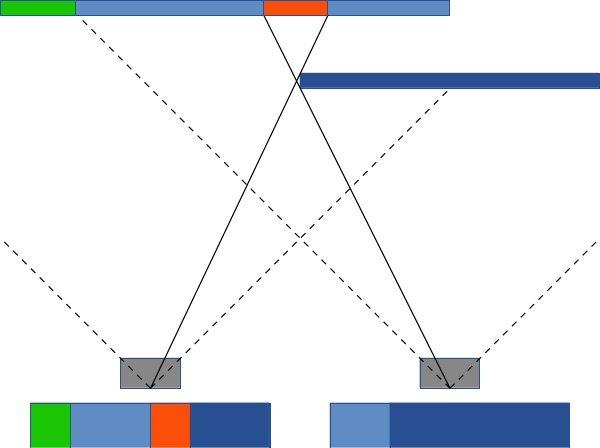
\includegraphics[width=0.5\textwidth]{images/borNParOcc}
  \caption{Example of border occlusion (green area) and partial non-border occlusion (orange area)}
  \label{fig:borNParOcc}
\end{figure}

\begin{figure}
  \centering
  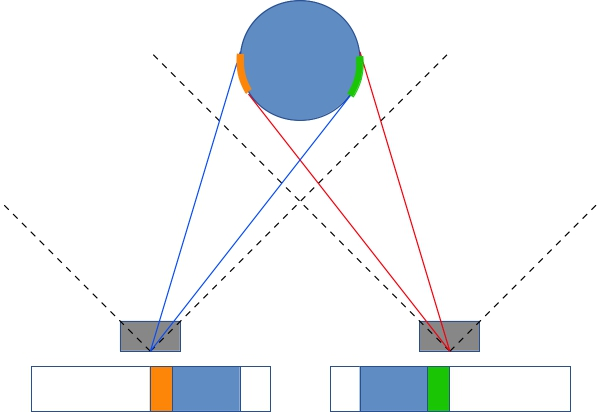
\includegraphics[width=0.5\textwidth]{images/selfOcc}
  \caption{Example of self non-border occlusion (green and orange area)}
  \label{fig:selfOcc}
\end{figure}

\begin{figure}
  \centering
  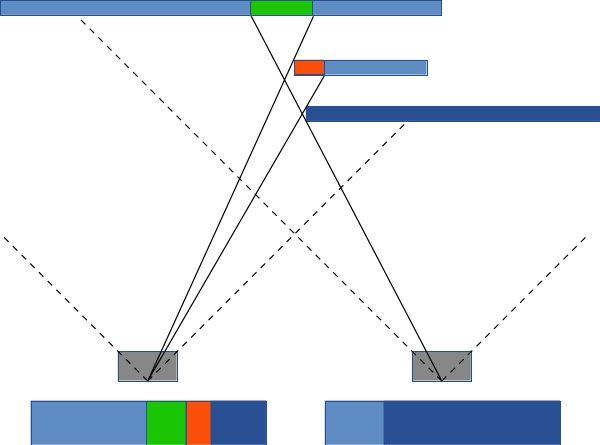
\includegraphics[width=0.5\textwidth]{images/compOcc}
  \caption{Example of total occlusion (orange area)}
  \label{fig:totalOcc}
\end{figure}

\textbf{Occlusion detection:}\\
Detecting occlusions can be done to ways: implicit and explicit. Implicit detection is when occlusions are handled while matching. Explicit detection is when the occlusions are detected by matching both ways. Currently the algorithm use explicit matching.\\
When occluded points are found then they are marked with a label or set to zero so the occluded area can be filled later.

\subsection{Occlusion filling}
This section will describe methods for filling the occluded areas. All these methods comes from the article: \textit{Occlusion filling in stereo: Theory and experiments} by \textit{Shafik Hyq, Andreas Koschan} and \textit{Mongi Abidi}. All these methods assume that the stereo matching is going from left image to right image i.e. templates are taken from the left image matched onto the right image.
 
\subsubsection{Neighbor's Disparity Assignment : NDA}
This is the simplest method to fill occlusions. It functions by selecting an occluded point, $p_L$, then find then nearest non-occluded point, $q_L$, to the left when filling non-border occlusion. With border occlusion the nearest point to the right is found instead. It is assumed that this non-occluded point is part of same surface as the occluded point (this can be seen on figure \ref{fig:borNParOcc}) and the disparity value from $q_L$ can be assigned to $p_L$. This method have some issues. In cases of total occlusions (see figure \ref{fig:totalOcc}) then a wrong disparity value is given to the total occluded object since it isn't a part of the nearest surface with non-occluded points to the left. In cases with self occlusions the occluded area should have disparity values close to the disparity values of the non-occluded points to the right (This will be the area of the surface which is in view of both cameras) but using NDA will give the occluded area disparity values corresponding to the background. 

\subsubsection{Diffusion in Intensity Space : DIS}
This method is inspired by diffusion. Diffusion is the movement of molecules or atoms from a high concentration region to a low concentration region. \\
After detecting occluded regions with cross-checking during template matching, the diffusion energy for the region is approximated. This method is depended on the stereo matching algorithm because it use the energy from the last iteration to determine initial diffusion energy for the area. \\
A change to the method can be made to make it independent from the stereo matching. The initial energy will be 0. Then the diffusion energy for non-border occlusion is found by:
\begin{equation}
E(p_L) = \min_{l_{p_L}=\{0,\dots, l_{max}\}} \left( \dfrac{1}{2 | q_L \in \mathcal{N}(p_L) \wedge l_{q_L=l_{p_L}} |} \; \sum_{q_L \in \mathcal{N}(p_L) \wedge l_{q_L = l_{p_L}}} (|\bar{I}(p_L)-\bar{I}(q_L) | + E(q_L))\right)
\end{equation}
And the diffusion energy for border occlusions are found by by:
\begin{equation}
E(p_L) = \min_{l_{p_L}=\{0,\dots, l_{p_{Lf}}-2\}} \left( \dfrac{1}{2 | q_L \in \mathcal{N}(p_L) \wedge l_{q_L=l_{p_L}} |} \; \sum_{q_L \in \mathcal{N}(p_L) \wedge l_{q_L = l_{p_L}}} (|\bar{I}(p_L)-\bar{I}(q_L) | + E(q_L))\right)
\end{equation}
The diffusion energy will be calculated for each occluded point and for each point the disparity which corresponds the minimum $E(p_L)$ is set as the disparity $l_{p_L}$ for the occluded point. 


\subsubsection{Weighted Least Squares : WLS}
In this approach, WLS, all the non-occluded and filled occluded neighbors in a neighborhood around the occluded point is considered valid points and is used as control points in interpolation.\\
Since the neighborhood contains both foreground points and background points and the occluded point is expected to be a part of the background then the background points should have more influence than foreground points. It is assumed that the color intensity between objects is significantly different and this property can be used to distinguish between foreground points and background points. \\
Each error term in the aggregated residual should be weighted so the foreground don't have much influence. With this the aggregated residual is defined as:
\begin{equation}
  \Delta = \sum_{q_L \in \mathcal{N}(p_L)} w_{q_L} (\hat{l}_{p_L}(p_L)-l_{p_L}(q_L))^2
\end{equation}
where $w_{q_L} = e^{-\mu_L | \bar{I}(p_L) - I(q_L)|}$ (the weight) is the likelihood of $p_L$ with $q_L$ under the assumption of an exponential distribution model of $| \bar{I}_(p_L)- I(q_L) |$. $\bar{I}(p_L)$ is the mean intensity of $p_L$ and $\mu_L$ is the decay rate. $\hat{l}_{p_L}(p_L)$ is the estimated disparity of $p_L$ (will be estimated during interpolation) and $l_{p_L}(q_L)$ is the disparity of $q_L$. \\
How to estimate $\bar{I}(p_L)$ and $\mu_L$:\\
$\bar{I}(p_L)$ is the mean intensity of $p_L$ which can be obtained using mean shift algorithm in a window around $p_L$. To estimate this value the initialize the algorithm with $\bar{I}(p_L) $ equal to the intensity of $p_L$ then the mean shift algorithm repeatedly picks those neighbors inside the window that satisfy $| \bar{I}(p_L) - I (q_L) | \geq 3\mu^{-1}$ and the assign the average of intensities of the selected neighbors to $\bar{I}(p_L)$ until $\bar{I}(p_L)$ converges to a fixed average. $|\bar{I}(p_L) - I(q_L)|$ has decay rate $\mu_L$ which is related to the decay rate $\mu$ of the variable $|I(p_L) - I(q_L)|$ by $\mu_L^2 = \mu$.\\
A matrix containing all the coordinates:
\begin{equation}
F = \begin{bmatrix}
  x_1 & y_1 & 1 \\
  \vdots & \ddots & \vdots\\
  x_n & y_n & 1 
\end{bmatrix}
\end{equation}
Vector with the corresponding labels for the coordinates in $F$:
\begin{equation}
L = [l_1 \; \cdots \; l_N] 
\end{equation}
Linear model:
\begin{equation}
l_{p_L} = a + b x (p_L) + c y (p_L)
\end{equation}
Where $(x(p_L),y(p_L))$ is the coordinates of $p_L$ and $a$, $b$ and $c$ are the model parameters. \\
The weights for the control points can be express in a vector as:
\begin{equation}
w = [w_{q_{L1}} \; w_{q_{L2}} \; \cdots \; w_{q_{LN}}]'
\end{equation}
Then we compute two new matrices, $F_w$ and $L_w$:
\begin{flalign}
&& F_w &= diag(w)F && \\
&& L_w &= diga(w)L &&   
\end{flalign}
The model parameter vector:
\begin{equation}\label{eq:parvec}
P = [\, a \; b \; c \,]'
\end{equation}
By combining the equations above then the following equation is given: 
\begin{equation}
P = (F^T_wF_w)^{-1}F^T_wL_w
\end{equation}
With these equation the disparity of the occluded point can be estimated:
\begin{equation}
\hat{l}_{p_L} = [1 \; x(p_L) \; y(p_L)] P
\end{equation}

\subsubsection{Segmentation-based Least Squares : SLS}
Biggest difference between WLS and SLS is that SLS only uses non-occluded points as control points. The control points is a subset of the non-occluded neighboring points. The control points are segmented from the neighborhood by applying different constraints: visibility constraint, disparity gradient constraint and color similarity cues. \\
Sequence of operations: 
\begin{itemize}
\item Select an occluded point
\item Select control points from the neighborhood around the occluded point
\item Interpolate the disparity of the occluded point from the segmented control points 
\end{itemize}
$\mathcal{N}(p_L)$ is a set of non-occluded, neighboring points which will be use for control points in the interpolation. For points to be added to $\mathcal{N}$ then it needs to fulfill some constraints.\\
\textbf{Disparity gradient constraint:} In most cases the horizontal closest non-occluded point to the right, $p_{Lf}$, will be part of the foreground and the occluded should be a part of the background. In this cases every non-occluded point with a lower disparity than $p_{Lf}$ will be added to $\mathcal{N}$ hence the condition for added the point, $q_L$, will be $l_{q_L} < l_{p_{Lf}}$. If the foreground object is narrow then all the non-occluded neighboring points might be from the background and have the same disparity. Due to this a second condition have to be added to the constraint. The horizontal closest non-occluded point to the left will be called $p_{Lb}$ and a second condition is created: $| l_{p_{Lb}} - l_{q_L} | \leq 1$. When these conditions are combined the constraint can be defined as:
\begin{equation}
| l_{p_{Lb}} - l_{q_L} | \leq 1 \vee  l_{q_L} < l_{p_{Lf}}  
\end{equation}
\textbf{surface constraint:} It is assumed that $\mathcal{N}(p_L)$ will contain points from maximum 2 different surfaces (due to the small neighborhood). Some cases might contain a third surface but this is expected to occur very seldom and therefore it is disregarded. The point with the lowest disparity, $l_{min}$, is assumed to belong to one of the surfaces and the point with the highest disparity, $l_{max}$, is assumed to belong to the other surfaces. If $l_{max} - l_{min} \leq 1$ then it is assumed the all the points in $\mathcal{N}$ belongs to a single surfaces otherwise the points have to be segmented into 2 groups. The first group will contain all points which satisfies $| l-{max} - l_{q_L} | \leq 1$ and the other group will contain all the points which satisfies $| l-{min} - l_{q_L} | \leq 1$.
\textbf{Color constraint:} The average truncated color distance from the occluded point, $p_L$, to each of the two groups to determine which group the point belongs to. The average truncated color distance is found by:
\begin{equation}
D(p_L,\mathcal{N}_i(p_L) ) = \dfrac{1}{|\mathcal{N}_i(p_L)|} \; \sum_{q_L \in \mathcal{N}(p_L)} \psi (p_L,q_L) 
\end{equation}

\section{Result / conclusion from article}
The article performs some test using the 4 occlusion filling methods. For the tests Middlebury stereo images are used. The tests shows the percentage of errors when filling occlusions. The results shows that SLS performs best, DIS performs second best and WLS and NDA performs about the same. SLS during the test performed in the article runs rather slow: 3-10 min while WLS runs for only 10 seconds. SLS is faster than DIS and NDA is expected to be the fastest methods since it is the simplest method. In the conclusion it is theorized that the performance of SLS can be improved greatly by running estimations in parallel. \\
In this project either NDA or SLS will be used. NDA for the fastest result and SLS for a better result.

\section{Proposed algorithm}
For this project the following algorithm will be used. 

\subsection{Complexity of the algorithm}
bla requires bli multiplication etc.



%-----------------
%\textbf{Math:}
%\begin{itemize}
%  \item $p_L$: occluded point
%  \item $q_L$: neighboring points
%  \item $l_{P_L}(q_L)$: disparity of $q_L$
%  \item $\hat{l_{P_L}(p_L)}$: disparity of occluded found by interpolation
%  \item $w_{q_L}$: the likelihood of $p_L$ with $q_L$
%  \item $i(p_L)$: intensity of $p_L$  
%  \item $\bar{I}(p_L)$: mean intensity of $p_L$
%  \item $\mu _L$: decay rate
%  \item $F$ is the matrix of coordinates of all the control points 
%  \item $L$ is the vector of their corresponding labels.  
%  \item $w$ is the weight vector
%  \item $F_w = diag(w)F$
%  \item $L_w = diag(w)L$ 
%  \item $P$ is the parameter vector $P = [a \; b \; c]'$
%  \item $E(p_L)$ the diffusion energy
%  \item $\mathcal{N}(p_L)$: set of non-occluded neighbors of $p_L$ 
%  \item $l_{p_{Lf}}$ disparity of the horizontal closest non-occluded point to the right of $p_L$. Expected to be part of foreground, f for foreground
%  \item $l_{p_{Lb}}$: disparity of the horizontal closest non-occluded point to the left of $p_L$. Expected to be part of background, b for background
%  \item $\Delta I$: absolute difference
%  \item $\mu ^{-1}$: variance of $\Delta I $
%  \item $\zeta$: Normalizing factor
%  \item $\alpha$: exponential distribution
%  \item $P(\Delta I)$: mixture probability model
%  \item $H(p_L,q_L)$: Homogeneity
%  \item $\psi$: cut-off function
%  \item $D(p_L,\mathcal{N}_i(p_L))$: average truncated color distance
%  \item $S_0$ background surface 
%\end{itemize}